\documentclass[12pt,a4paper, ngerman]{article}
\usepackage{babel}
\usepackage{amsmath}
\usepackage[style=numeric]{biblatex}
\addbibresource{Maturarbeit.bib}
\usepackage{graphicx}
\usepackage{wrapfig}
\usepackage{listings}
\usepackage{xcolor}

\definecolor{codegreen}{rgb}{0,0.6,0}
\definecolor{codegray}{rgb}{0.5,0.5,0.5}
\definecolor{codepurple}{rgb}{0.58,0,0.82}
\definecolor{backcolour}{rgb}{0.95,0.95,0.92}
 
\lstdefinestyle{mystyle}{
    backgroundcolor=\color{backcolour},   
    commentstyle=\color{codegreen},
    keywordstyle=\color{magenta},
    numberstyle=\tiny\color{codegray},
    stringstyle=\color{codepurple},
    basicstyle=\ttfamily\footnotesize,
    breakatwhitespace=false,         
    breaklines=true,                 
    captionpos=b,                    
    keepspaces=true,                 
    numbers=left,                    
    numbersep=5pt,                  
    showspaces=false,                
    showstringspaces=false,
    showtabs=false,                  
    tabsize=2
}
 
\lstset{style=mystyle}

\begin{document}
\title{\large Maturitätsarbeit an der Kantonsschule Zürich Nord \\ \Huge Regelungstechnik \\ \huge PID-Parameter anhand einem Quadrocopter erforschen}
\date{\today}
\author{Charpoan Kong \\ M6d \\ Kantonsschule Zürich Nord}
\maketitle
\pagenumbering{gobble}





\newpage
\clearpage
\pagenumbering{gobble}
\tableofcontents
\newpage
\pagenumbering{arabic}

\section{Einleitung}
Ein Quadrocopter ist ein Flugobjekt mit 4 Propellern. In der Vergangenheit wurden schon Versuche mit Flugobjekten mit 4 Propellern gemacht z.B. wie der Luftfahrtpionier Étienne OEhmichen. der 1920 den Oehmichen No. 2 gebaut hatte. Damals waren die Propeller elastisch und man konnte mit Seilzügen den Anstellwinkel der Propeller einstellen. Er konnte damit einige Rekorde aufstellen.\cite{website:Wikipedia_Quadrocopter}\\

In der heutigen Zeit finden Quadrocopter viele Anwendungen, wie z.B. bei Suchaktionen, im Militär, oder auch als Spielzeug. Mit der schnellen entwicklung von Mikroprozessoren wurden Quadrocopter immer kleiner und einfacher zu realisieren. Auch können damit teurere Helikopterflüge für Kartographie oder Luftaufnahmen billiger realisiert werden.\\

Mit dieser Arbeit will ich mit dem Bau und dessen Regelung befasssen. Der Quadrocopter wird selbst gebau mit dem Hauptziel den Flightcontroller selbst zu designen, bauen und programmieren. So sollte die Regelung selbst implementiert werden. Dannach sollten Versuche gemacht werden, die bestimmen sollten, wie der PID-Regler stabiler gemacht werden kann und wie ungleichheiten, wie sie durch Vibration entstehen, auszugleichen.
\newpage
\section{Was ist ein Quadrocopter?}
Ein Qadrocopter ist wie in der Einleitung beschrieben ein Flugobjekt. Man könnte meinen, dass man einen stabilen Flug erreichen kann, wenn man den vier Propellern den gleichen Schub gibt. Aber dies ist leider nicht möglich, da viele Umwelteinflüsse einen stabilen Zustand verhindern wie z.B. Wind, unterschiede in den Rotoren oder Motoren, assymetrie des Rahmens etc. So muss ein Computer, der Flightcontroller(FC), das Gleichgewicht erhalten, indem dieser den Schub der vier Motoren so steuert das der Quadrocopter im Gleichgewicht ist oder dieser einen anderen bestimmten Winkel hält.\\
\begin{figure}[h]
\centering
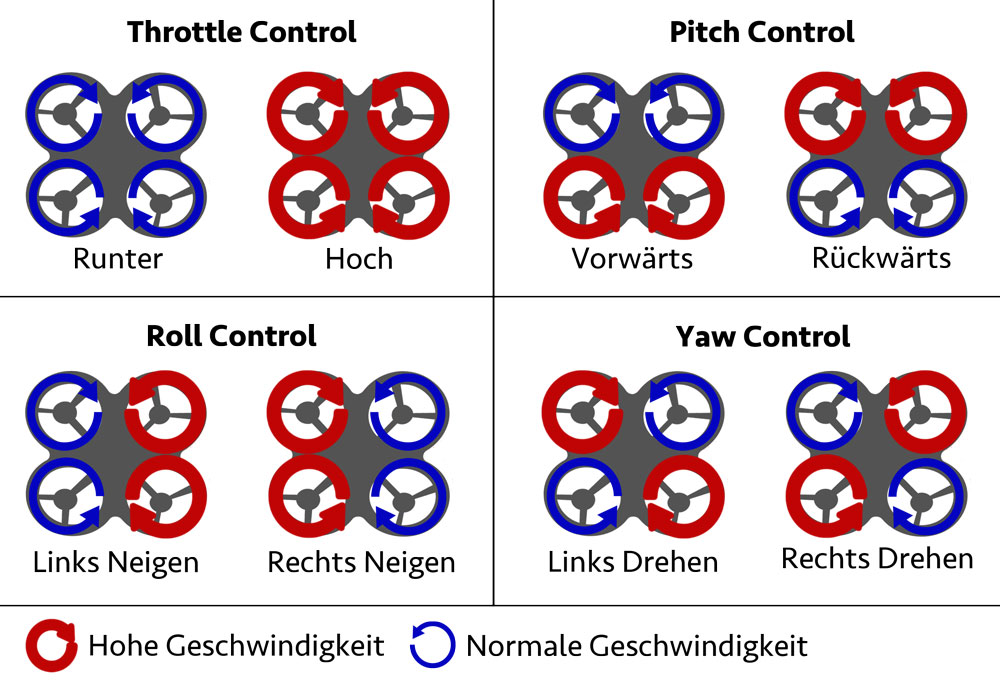
\includegraphics[width=\textwidth]{MotionDE.jpg}
\caption[https://fpvracing.ch/de/content/7-grundsatzliche-funktion-quadrocopter-multicopter]{Drehrichtung und Schub bei verschiedenen Steuereingaben }
\end{figure}\\
Man sieht in dieser Abbildung welche Rotationsrichtung die Motoren haben. Die benachbarten Motoren müssen eine gegensätzliche rotation haben, da sonst der Quadrocopter zum rotieren kommt. So wird das Drehmoment des anderen Motors ausgeglichen. Auch wird gezeigt, dass man den Quadrocopter mit erhöhen bzw. erniedrigen der Motorleistung der richtigen Motoren, diesen in die gewünschte Richtung steuern kann. Der FC hält dieses Gleichgewicht mit einem Proportional-,Integral- und Differenzial-Regler(PID-Regler).


\section{PID-Regler und Filter}
\subsection{Was ist ein Regler?}
Eine Regelung ist ein Steuerung mit Rückkoppelung. Es wird ein Wert z.B. die Drehzahl eines Motors überwacht und je nach gewünschter Drehzahl, das Drehmoment des Motors geregelt, dass er auch diesen halten kann, auch wenn eine Last am Motor hängt.\cite{website:rn-wissen_Regelungstechnik}\\
\begin{wrapfigure}[6]{r}{0.4\textwidth}
\centering
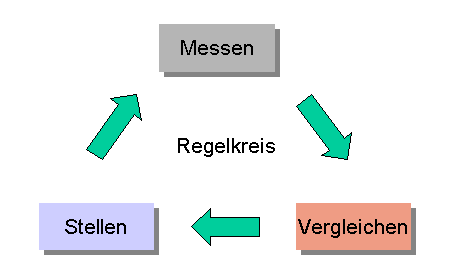
\includegraphics[width=0.4\textwidth]{Regelkreis1.png}
\caption[https://rn-wissen.de/wiki/images/2/25/Regelkreis1.png]{Der Regelkreis}
\end{wrapfigure}
Der Regelkreis misst die Regelgrösse z.B. mit einem Sensor. Dann wird dieser mit dem Soll-Wert verglichen um die Regelabweichung zu bestimmen. So kann ein z.B. Motor gestellt werden damit dieser sich dem Soll-Wert nähert.\\ \\ \\ \\

Die Regelabweichung kann dabei einfach mit der Differenz des Ist-Wertes $x$ mit dem Soll-Wertes $w$ bestimmt werden.
\begin{equation}
e(t)=w-x
\end{equation}
\begin{wrapfigure}[8]{l}{0.4\textwidth}
\centering
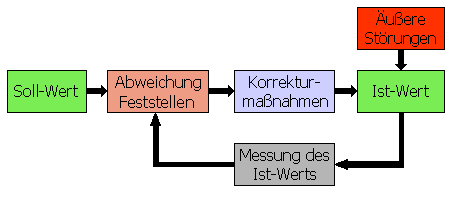
\includegraphics[width=0.4\textwidth]{Regelkreis2.png}
\caption[https://rn-wissen.de/wiki/images/5/5d/Regelkreis2.png]{Wirkungsweise des Regelkreises}
\end{wrapfigure}
In der Abbildung 3 sieht man, wie vorher beschrieben, wie ein solcher Regelkreis funktionert. In der Regelungstechnik wird versucht einen solchen Regelkreis mathematisch zu modellieren. In dem Kapitel wird nur der PID-Regler und seine Komponenten besprochen, da dieser häufig bei Quadrocoptern benutzt wird.
\\ \\ \\
Der PID-Regler besteht aus mehreren Relgern und dem D-Glied. Untern wird beschrieben wie die einzelnen Komponenten wirken. 

\subsubsection{P-Regler}
Der P-Regler wirkt linear. Dieser Regler gibt die Regelabweichung verstärkt und unverzögert mit dem Faktor $Kp$ weiter. Das Problem dabei ist, dass diese Abweichung bleibend ist und somit den Soll-Wert über- bzw. unterschiesst. Dieser Regler wirkt mittelschnell.\cite{website:rn-wissen_Regelungstechnik}\\
\begin{equation}
y(t)=Kp*e(t)
\end{equation}
\begin{lstlisting}[language=C++,caption=P-Regler C++ Pseudocode]
void P_Regler(float Kp, float error, float &P){
	P = kp * error;
}
\end{lstlisting}

\subsubsection{I-Regler}
Beim Integralregler wird die Regelabweichung über die Zeit summiert und mit dem Faktor $Ki$ verstärkt. Dabei werden Abweichungen volständig eliminiert, da dieser Regelwert immer anwächst solange die Regelabweichung nicht Null ist. Dieser Regler wirkt langsam.\cite{website:rn-wissen_Regelungstechnik}\\
\begin{equation}
y(t)=Ki\int_{0}^{t}e(t)dt
\end{equation}
\begin{lstlisting}[language=C++,caption=I-Regler C++ Pseudocode]
void I_Regler(float Ki, float error, float &I ){
	I += I+error*Ki;
}
\end{lstlisting}

\subsubsection{D-Glied}
Das Differenzialglied schaut auf die Differenz der Regelabweichung zur vorherigen Regelabweichung und wird mit dem Faktor $Kd$ verstärkt. Desshalb reagiert dieser sehr schnell und gibt den den beiden anderen Vorhaltezeit. Differenzialglied ist kein Regler da es alleine nichts regleln kann sondern nur auf Veränderungen in der Regelabweichung reagiert.\cite{website:rn-wissen_Regelungstechnik}\\
\begin{equation}
y(t)=Kd*e(t)\frac{d}{dt}
\end{equation}
\begin{lstlisting}[language=C++,caption=D-Regler C++ Pseudocode]
void D_Glied(float Kd, float error, float &previous_error, float dt, float &D){
	D = Kd * (error - previous_error);
	previous_error = error;
}
\end{lstlisting}

\subsubsection{PID-Regler}
Beim PID-Regler werden die Eigenschafter der einzelnen Regler und dem D-Glied vereint.
\begin{equation}
y(t)=Kp*e(t)+Kd*e(t)\frac{d}{dt}+Kd*e(t)\frac{d}{dt}
\end{equation}
\begin{lstlisting}[language=C++,caption=D-Regler C++ Pseudocode]
void PID_Regler(float P, float I, float D, float &PID){
	PID = P + I + D;
}
\end{lstlisting}
\subsection{Digitaler Low-Pass Filter}
Ein Low-Pass Filter filtert hohe Frequenzen aus. Man kennt diesen Filter meist aus der Elektronik oder der Tontechnik. Beim Quadrocopter wird ein solcher Filter für das unterdrücken des Rauschens der IMU verwendet. Dieses Rauschen wird durch die Vibrationen der Motoren erzeugt und liegt ca. bei 133Hz.\\ \\
Beim Digitalen Low-Pass Filter(DLPF) wird ein analoger RC-Low-Pass Filter emuliert.
Herleitung? \\ \\ 
Vibrationen verursachen beim D-Glied starke auschläge, wenn diese hohe Amplituden haben. Auch wird dieser dann unbrauchbar, da die Regelabweichung durch die Vibrationen verfälscht wird.
\newpage
\section{Äusserer Aufbau}
\subsection{Motoren}
Die verwendeten Motoren sind sogenannte bürstenlose Motoren. Diese werden mit einem Electronic Speed Controller(ESC) angesteuert, da diese wie Drehstrommotoren funktionieren. Da ihre RPM von Spannung abhängig ist gibt man noch einen $Kv$-Wert an. So kann man mit der Formel
\begin{equation}
RPM=Kv*U
\end{equation}
die Rotationen pro Minute berechnen.\\ \\
Beim meinem Quadrocopter handelt es sich um ReadyToSky RS2205 Motoren mit einem $Kv$ von 2300. Ich habe diese Motoren ausgesucht, da sie für genug Leistung bringen für einen Quadrocopter mit einer Rahmen länge von 250mm.(Bild l)
\subsection{Akku}
Der Akku versorgt alle Kompionenten, die Strom brauchen mit Strom. Im Quadrocopter wird ein LiPo Akku benutzt, der drei Zellen in Serie geschaltet hat mit einer Kapazität von 2.4Ah. Die miminale Spannung beträgt 11.1V. Es gibt noch das Entladerate, die als $C$-Rate angegeben wird. Mit mit der Kapazität multipliziert gibt es den maximalen Entladestrom an.\cite{website:fpvracing.ch_Mult_Komp}
\begin{equation}
A_{max}=Q*C
\end{equation} (Bild r)\\ \\
Man benutzt in Quadrocoptern meist LiPo Akkus, da sie eine hohe Energiedichte besitzen und viel Leistung abgeben können. Das aber hat auch zur Folge, dass man diese Akkus sorgfältig behandeln muss, da sie auch. im Extremfall, Feuer fangen oder explodieren können. So darf man die einzelnen Zellen nicht unter einer Spannung von 2.7V bringen. Desshalb wird der Akku auch an einem Akkuüberwacher angeschlossen, der piepst, wenn der Akku verbraucht ist. Auch braucht man ein Balancerladegerät, das kontrolliert, dass alle Zellen gleichmässug geladen werden. Eine hohe Kapazität garantiert nicht immer eine längere Flugzeit, da mehr Kapazität auch mehr Gewicht bedeutet.
\newpage

\section{Der Flightcontroller}
Der Flightcontroller ist das Herz des Quadrocopter er liest alle Sensoren und gibt den ESCs die Steuerimpulse. In dem Kapitel wird zuerst in die wichtigsten Komponenten eingegangen, dann wird der Design-, Bau und Propgrammierprozess beschrieben.
\subsection{Komponenten}
\subsubsection{Microcontroller}
Der Microcontroller der auf dem FC benutzt wird ist ein ARM-Cortex-M7 STM32F722RET6 Microcontroller von STMicroelectronics. Dieser besitzt alle Schnittstellen um die einzelen Sensoren und andere Komponenten auszulesen und anzusteuern. Da dieser nicht genug Pins hat, wird noch ein zweiter Microcontroller benutzt und zwar der ATMega328P, der auch auf dem Arduino/Genuino UNO zu finden ist. Dieser liest den Drucksensor und einige ADCs aus und kommuniziert mit dem I2C-Protokoll mit dem STM32. \\ \\
Microcontroller können anders als Mikroprozessoren ohne Zusatz Pehpetrie benutzt werden, da sie schon einen Flash, RAM etc. besitzen. Aber dies kommt mit einer tieferen Taktrate daher. Dies stört aber den Quadrocopter ist da diese völlig ausreichend ist. Der Hauptcontroller lauft mit einer Taktfrequenz von 200MHz.

\subsubsection{Sensoren}
Die wichtigsten Sensoren des Quadrocopter sind der Gyrosensor und der Beschleunigungssensor. In dem FC wurde eine ICM-20689 von TDK InvSense benutzt. Dieser hat beide Sensoren in einem Chip integriert und wird per SPI-Protokoll ausgelesen. Als Backup wird ein MPU-6050 benutzt, auch vom gleichen Hersteller, dieser wird mit dem langsameren I2C-Protokoll ausgelesen. \\

\begin{wrapfigure}[6]{r}{0.5\textwidth}
\centering
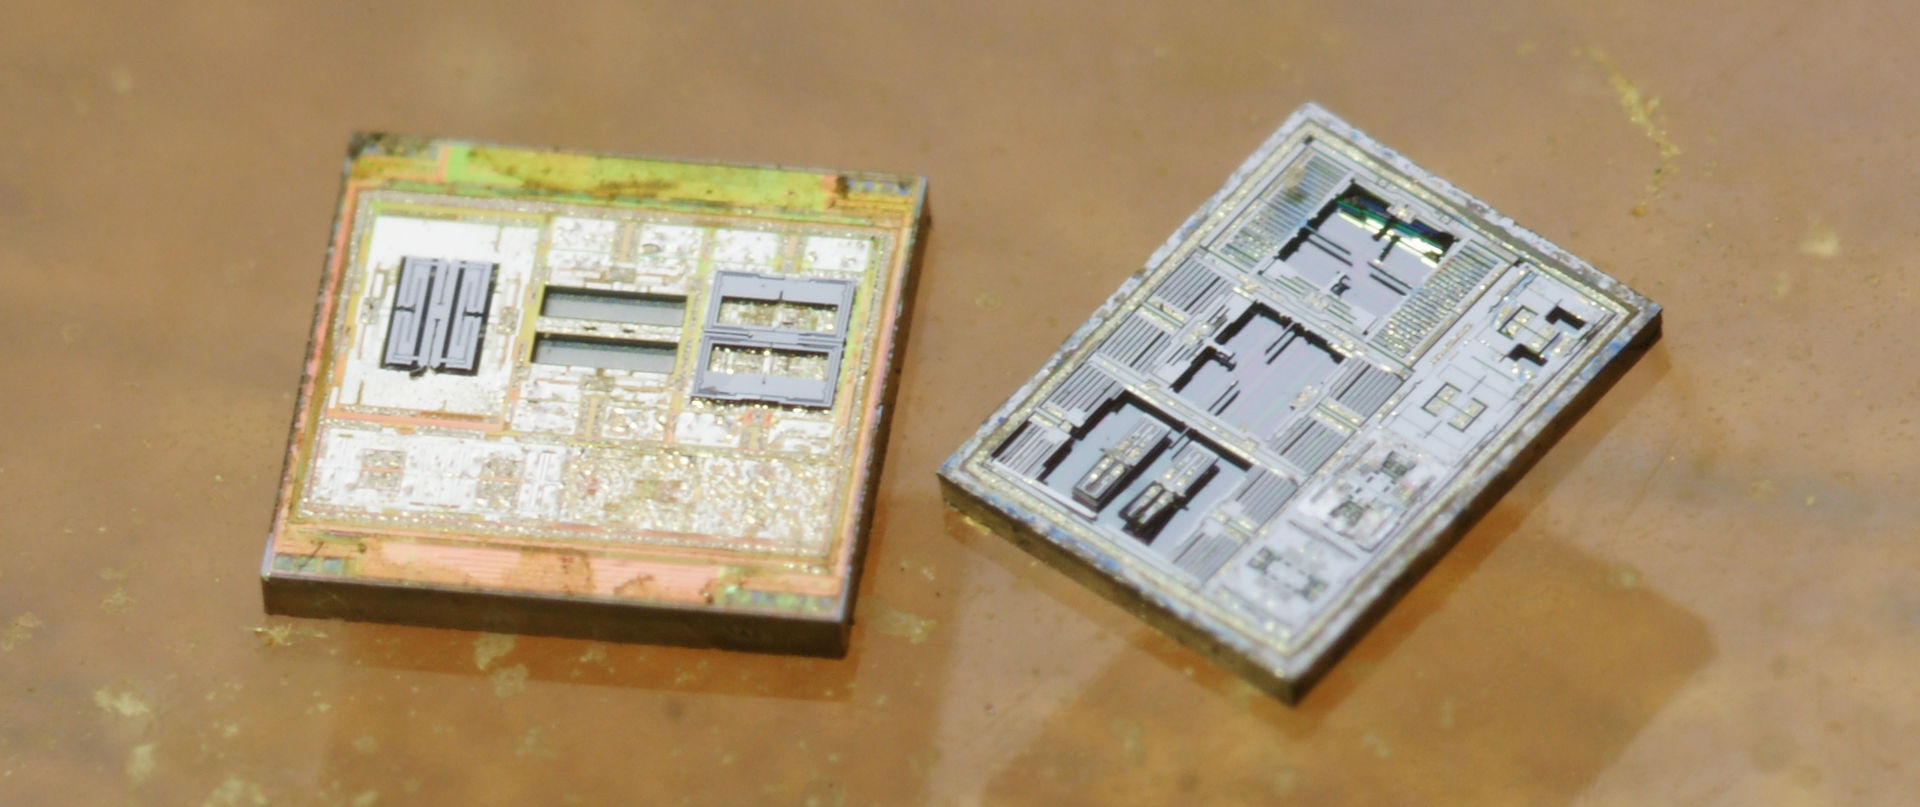
\includegraphics[width=0.5\textwidth]{1920px-Mpu6050-HD.jpg}
\caption[https://de.wikipedia.org/wiki/TDK]{Dice des MPU6050}
\end{wrapfigure}
Beide sind sogenannte MEMS-Sensoren, diese werden Direkt auf den Siliziumwaver der Chips realisiert. (Bild) Man ätzt die Sensorstrukturen und deren auslese Schaltung auf einen Chip. 
\newpage
Da der Gyrosensor nur Winkelgeschwindigkeit, bei den Sensoren $\frac{^\circ}{s}$ und nicht $\frac{rad}{s}$ misst muss diese noch mit der Loop-Zeit verrechnet werden um den Winkel zu bekommen.
\begin{equation}
Grad=\omega*dt
\end{equation}
Wenn man den Absoluten Winkel alleine mit dem Gyrosensor misst hat dieser in der Zeit einen Drift. Zum einen wird das durch das Rauschen im Sensor verurasacht und zu anderen auch von einem nicht genauen Loop-Zeit. Auch kann nicht der Anfangswinkel bestimmt werden und man müsste den Quadrocopter immer vom Boden aus starten. Deswegen braucht man da den Beschleunigungssensor. Dieser misst die Beschleunigung auf allen Achsen relativ zur Erdbeschleunigug. Beim Stillstand misst er also
$
\begin{pmatrix}
0\\ 
0\\ 
1
\end{pmatrix}
\vec{g}
$. Man kann einfach die Norm des Vektors nehmen und mit der Beschleunigung an der gewünschten Achse verrechnen um dann den Winkel zu bekommen.
\begin{equation}
Grad=
\left \|
\begin{pmatrix}
a_{x}\\ 
a_{y}\\ 
a_{z}
\end{pmatrix}
\right \|
\vec{g}*\frac{180}{\pi}
\end{equation}
So hat man den absoluten Winkel mit zwei Sensoren gemessen und muss diese nur noch Kombinieren. Dies geschieht mit der Formel des Komplementärflilters. Man muss auch beachten das man nur den Absoluten Winkel nur für die Nick-und Rollachse berechnen kann da, für die Gierachse noch ein Magnetometer nötig wäre für eine Null-Referenz.
\begin{equation}
Grad_{komp}=0.96*Grad_{Gyro}+0.04*Grad_{Accl}
\end{equation}
Man gibt dem Winkel aus dem Beschleunigungssensor einen tiefen Faktor da dieser Winkel nicht mehr genau stimmen wird, wenn der Quadrokopter in eine Richtung beschleunigen würde, dies wird erst bei starken Beschleunigungen der Fall sein, sonst stimmt dieser Wert ungefähr. Aber so kann man den Anfangswinkel des Quadrokopter bestimmen, ihn auch aus der Hand starten lassen und bekommt auch noch stabilere Werte. (Barometer ?) 

\subsubsection{Empfänger}
Als Empfänger wir dein NRF24L01 Breakoutboard mit PA und LNA benutzt. Der ist ein 2.4GHz Sender und Empfänger von der Firma Nordic Semiconductor. Die Kommunikation erfolgt digital und der Chip besitzt auch eine Zyklische Redundanzprüfung(CRC). Damit wird kontrolliert, ob ein Datenpaktet fehlerhafte Bits besitzt. Allenfalls wird es repariert oder verworfen. PA heisst Power Amplifying und bedeutet, dass das Signal verstärkt wird und so grössere Reichweiten erreicht werden können und LNA bedeutet Low Noise Amplifying und beseutet, dass schwache Empfangssignale verstärkt werden.\cite{website:electronics.stackexchange.com_WhatisPALNA} Vom Hersteller wird eine Reichweite vom bis zu einem Kilometer versprochen aber in einer Wohnsiedlung kommt man mit Sichtkontakt bis zu 300m, was ausreichend genug ist.

\subsubsection{Schnitstellen}


\subsection{Leiterplatte}

\subsubsection{Design}

\subsubsection{Bau}

\subsection{Programmierung}

\subsubsection{Motoren und Timing}

\subsubsection{PID Implementierung}

\section{Fernbedienung}

\section{Versuche}

\subsection{PID absoluter Winkel oder Winkelgeschwindigkeit}

\subsubsection{Absoluter Winkel}

\subsubsection{Winkelgeschwindigkeit}

\subsubsection{Ergebnisse}

\subsection{Filter}

\subsubsection{Ohne Filter}

\subsubsection{Filter 1}

\subsubsection{Filter 2}

\subsubsection{Ergebnisse}

\section{Schlussfolgerung}




\newpage
\section{Glossar}


\newpage
\section{Quellenverzeichnis}
\subsection{Literaturverzeichnis}
\printbibliography
\subsection{Abbildungsverzeichnis}
\listoffigures
\subsection{Personenverzeichnis}

\end{document}
